\section{Experimental results}
\subsection{Synthetic data set experiments}
\begin{frame}{On synthetic data set}
Setup
\begin{itemize}
\item Two normal classes data: 250 samples of each
\item A ring-like Outlier data set: 150 samples
\item Given different sets of data labels
\end{itemize}
\end{frame}
\begin{frame}{Results I}
Given 5 outliers / 15 outliers...
\begin{figure}
\centering
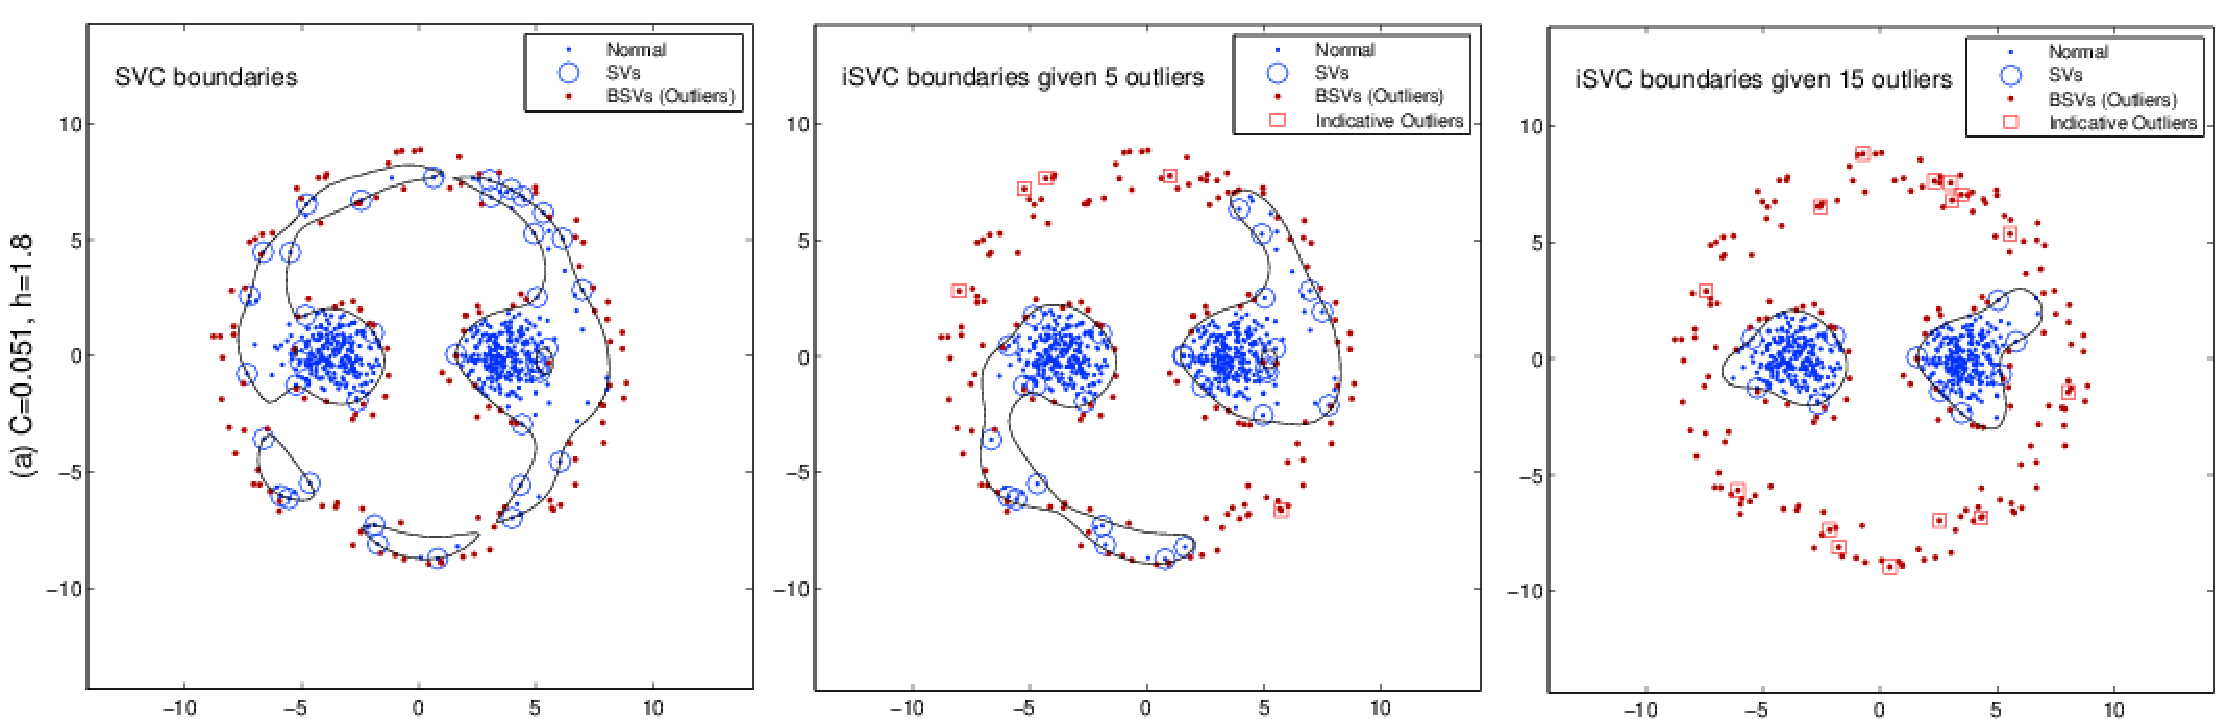
\includegraphics[scale=0.28]{imgs/syn_01_01.pdf}\\
%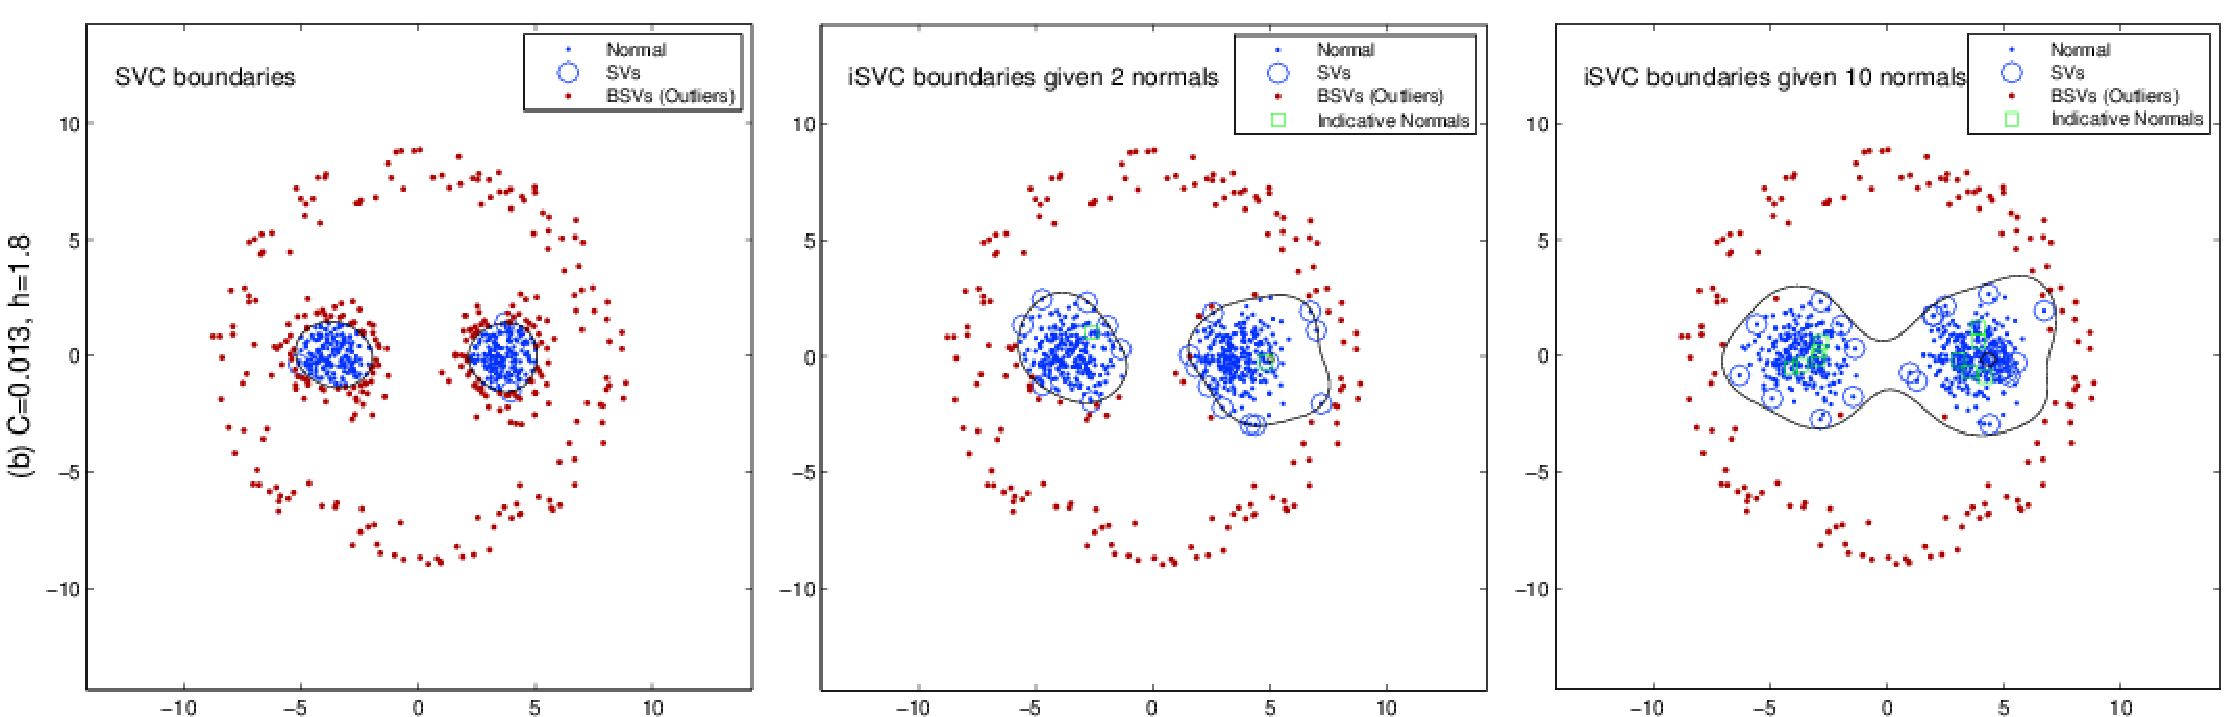
\includegraphics[scale=0.5\textwidth]{imgs/syn_01_02}\\
%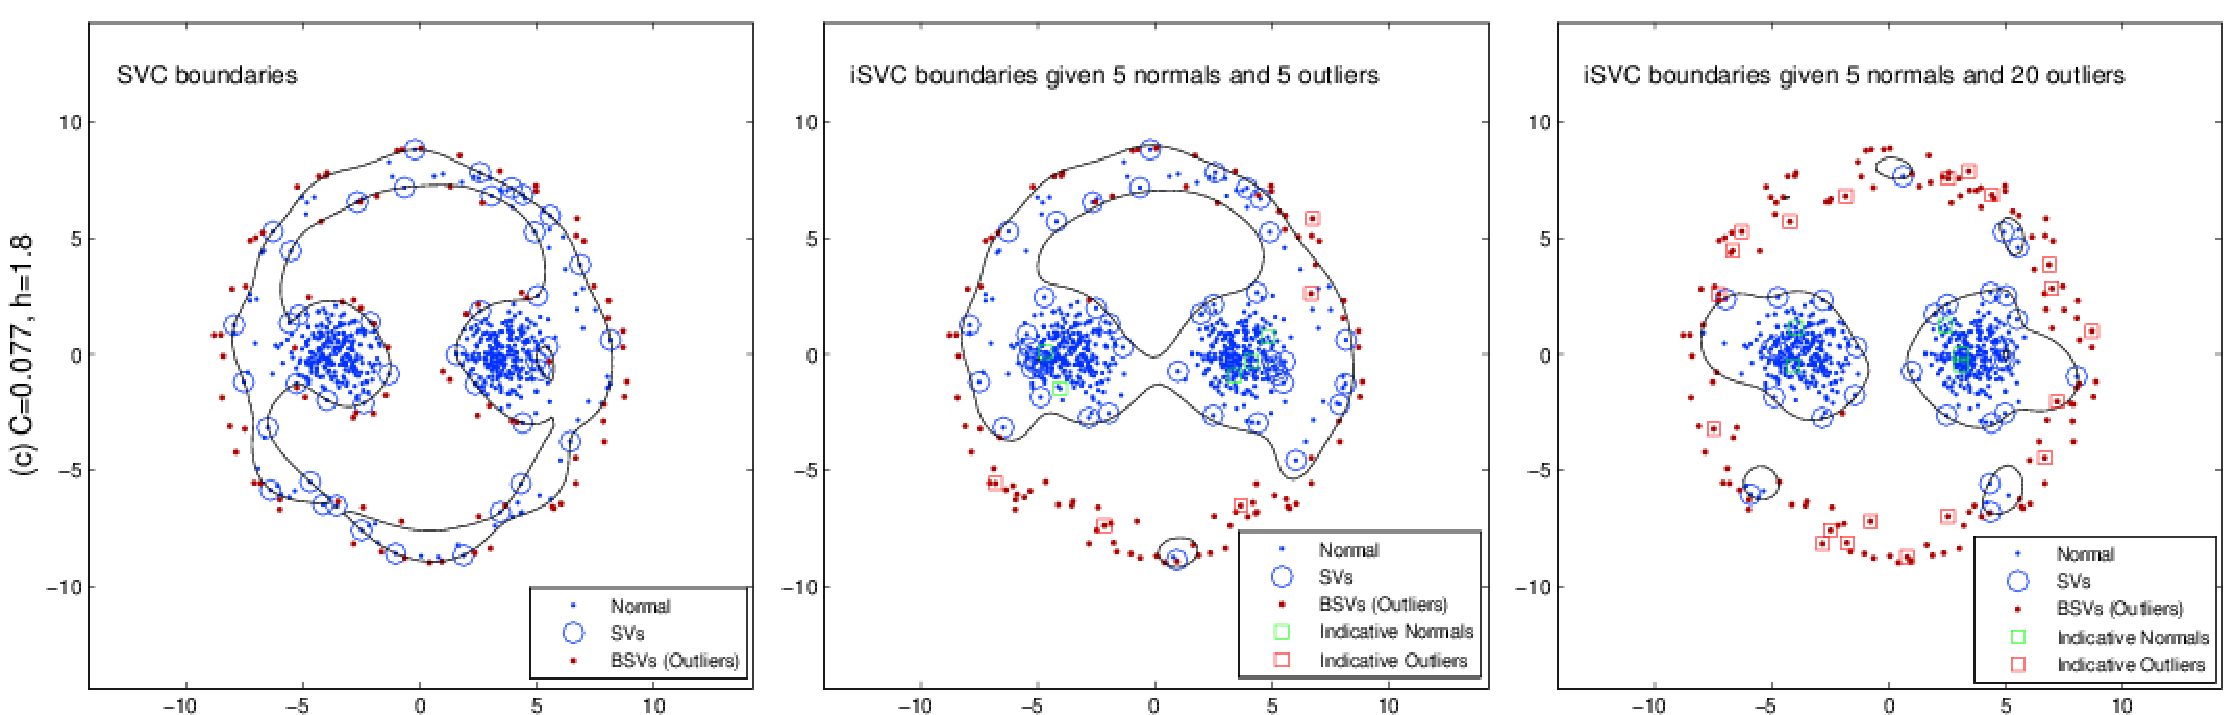
\includegraphics[scale=0.5\textwidth]{imgs/syn_01_03}
\end{figure}
\end{frame}
\begin{frame}{Results II}
Given 2 Normals / 10 Normals...
\begin{figure}
\centering
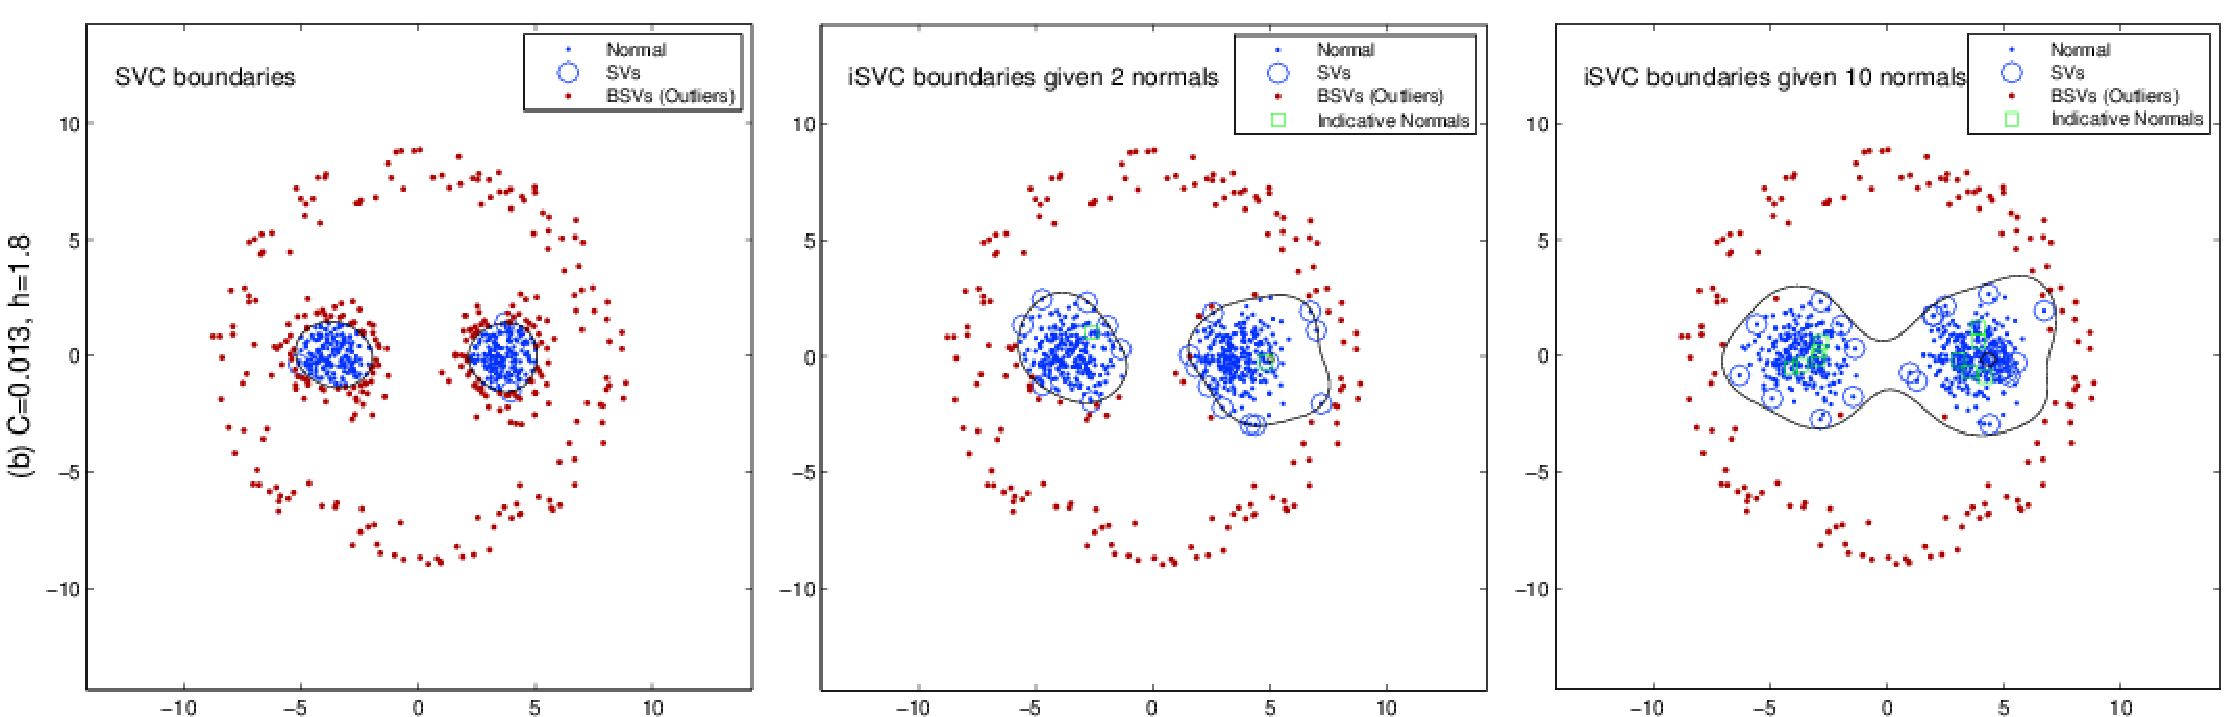
\includegraphics[scale=0.28]{imgs/syn_01_02.pdf}\\
%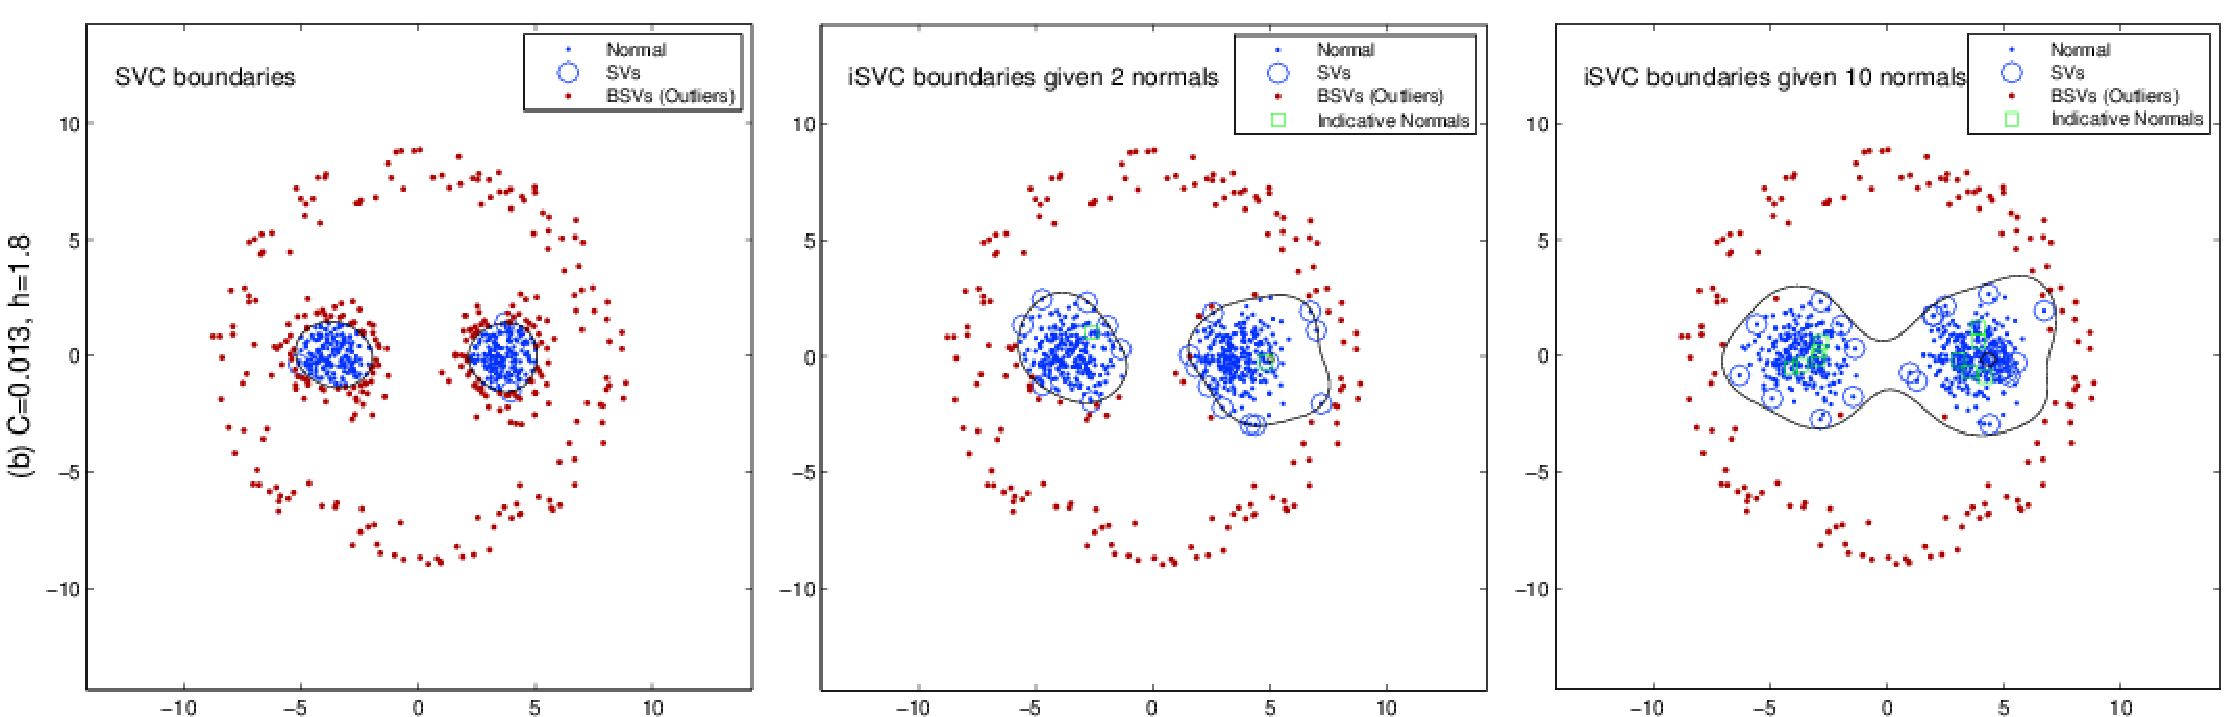
\includegraphics[scale=0.5\textwidth]{imgs/syn_01_02}\\
%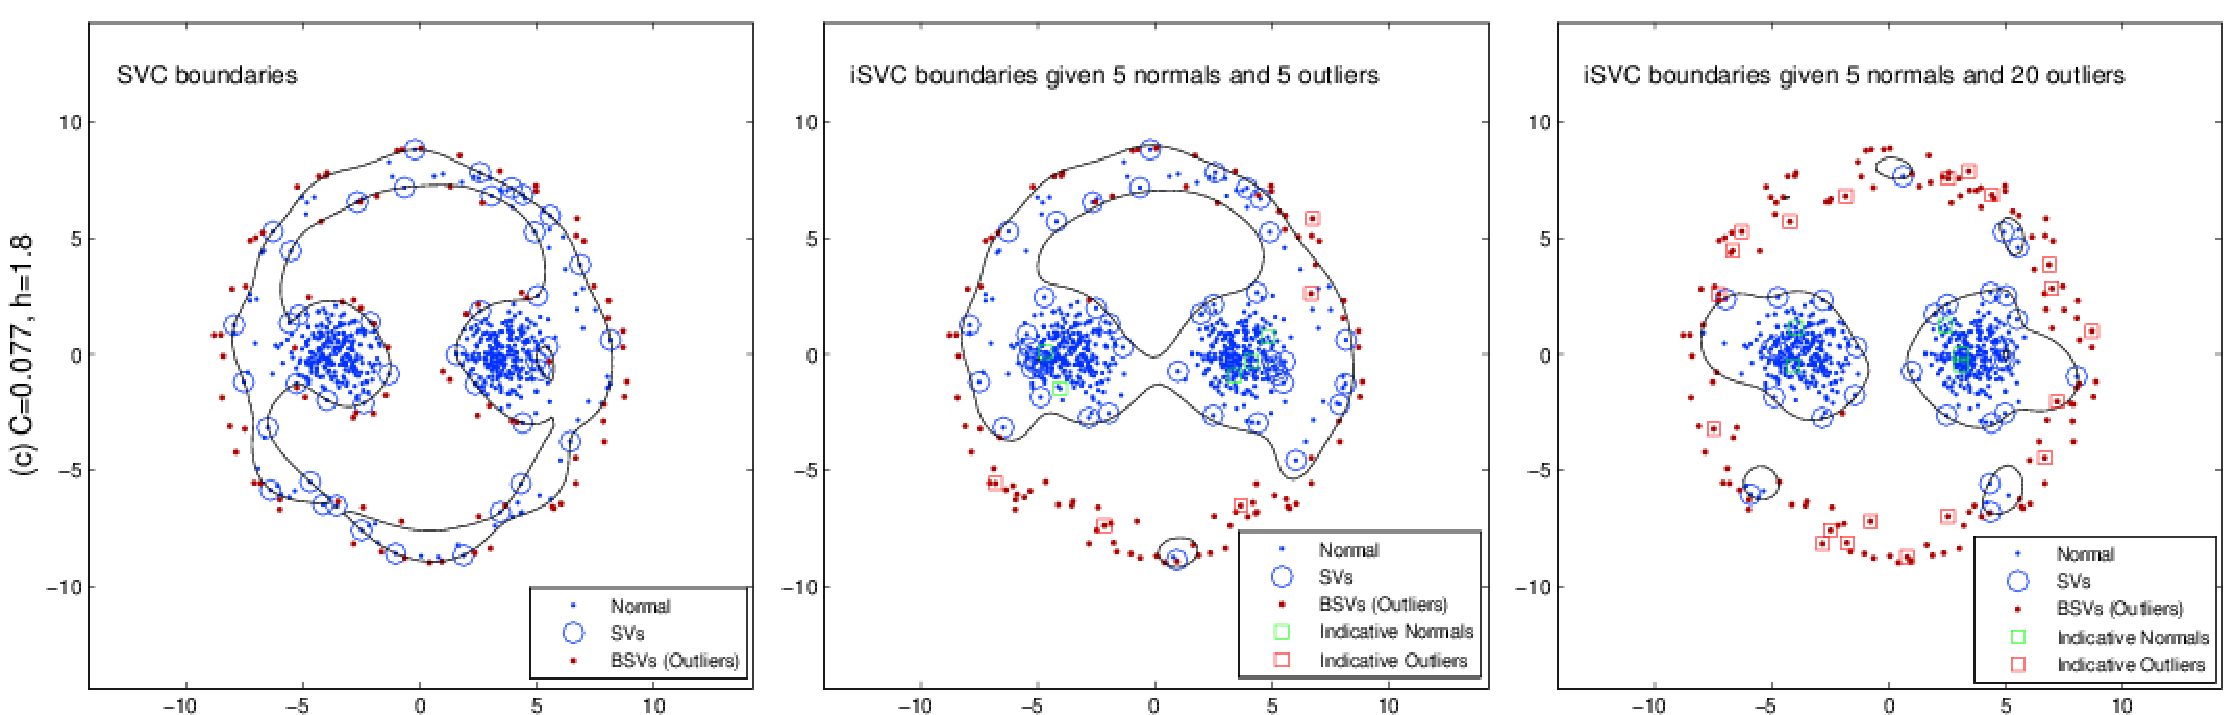
\includegraphics[scale=0.5\textwidth]{imgs/syn_01_03}
\end{figure}
\end{frame}
\begin{frame}{Results III}
Given 5 Normals and 5 Outliers / 5 Normals and 20 outliers...
\begin{figure}
\centering
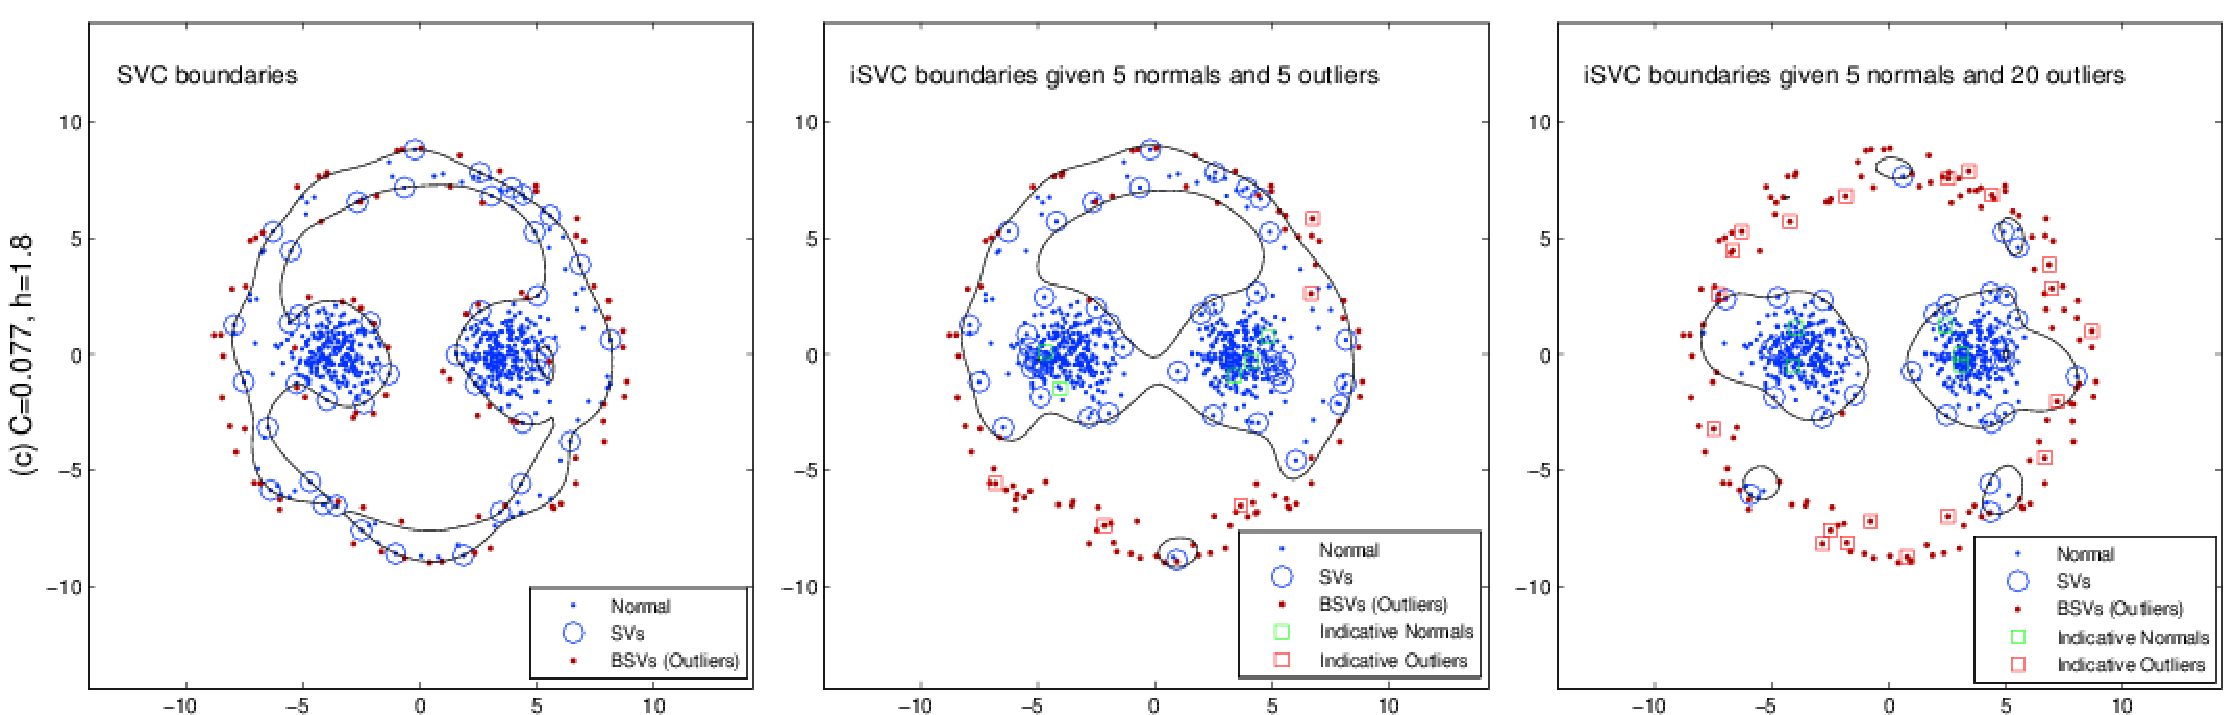
\includegraphics[scale=0.28]{imgs/syn_01_03.pdf}\\
%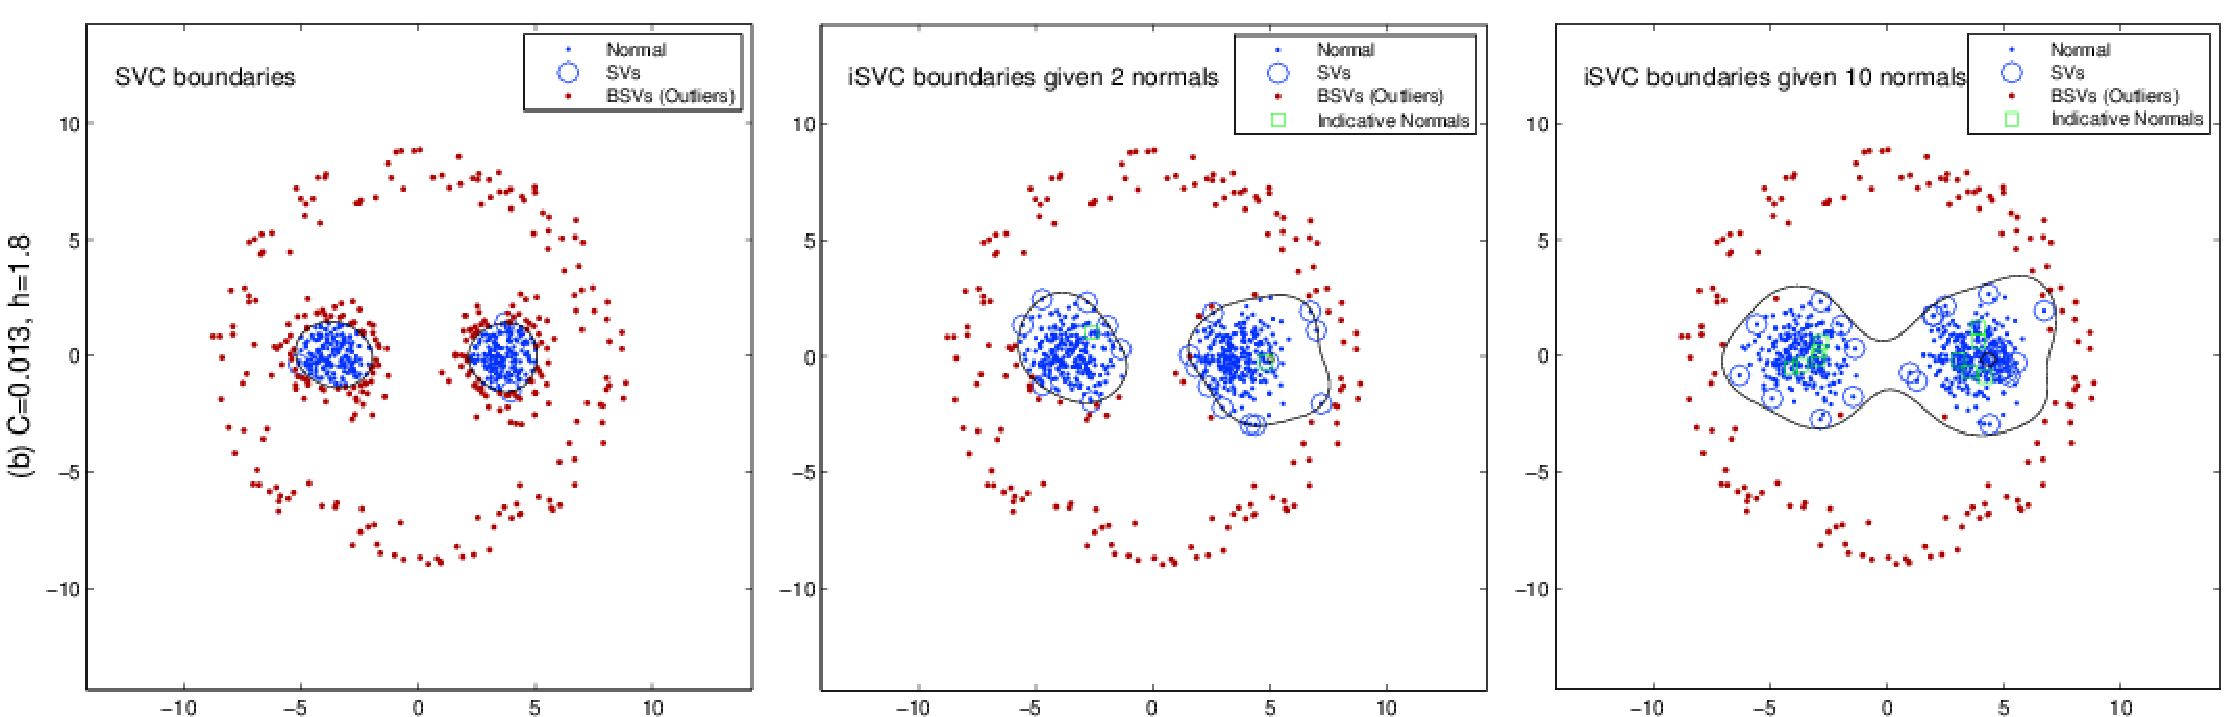
\includegraphics[scale=0.5\textwidth]{imgs/syn_01_02}\\
%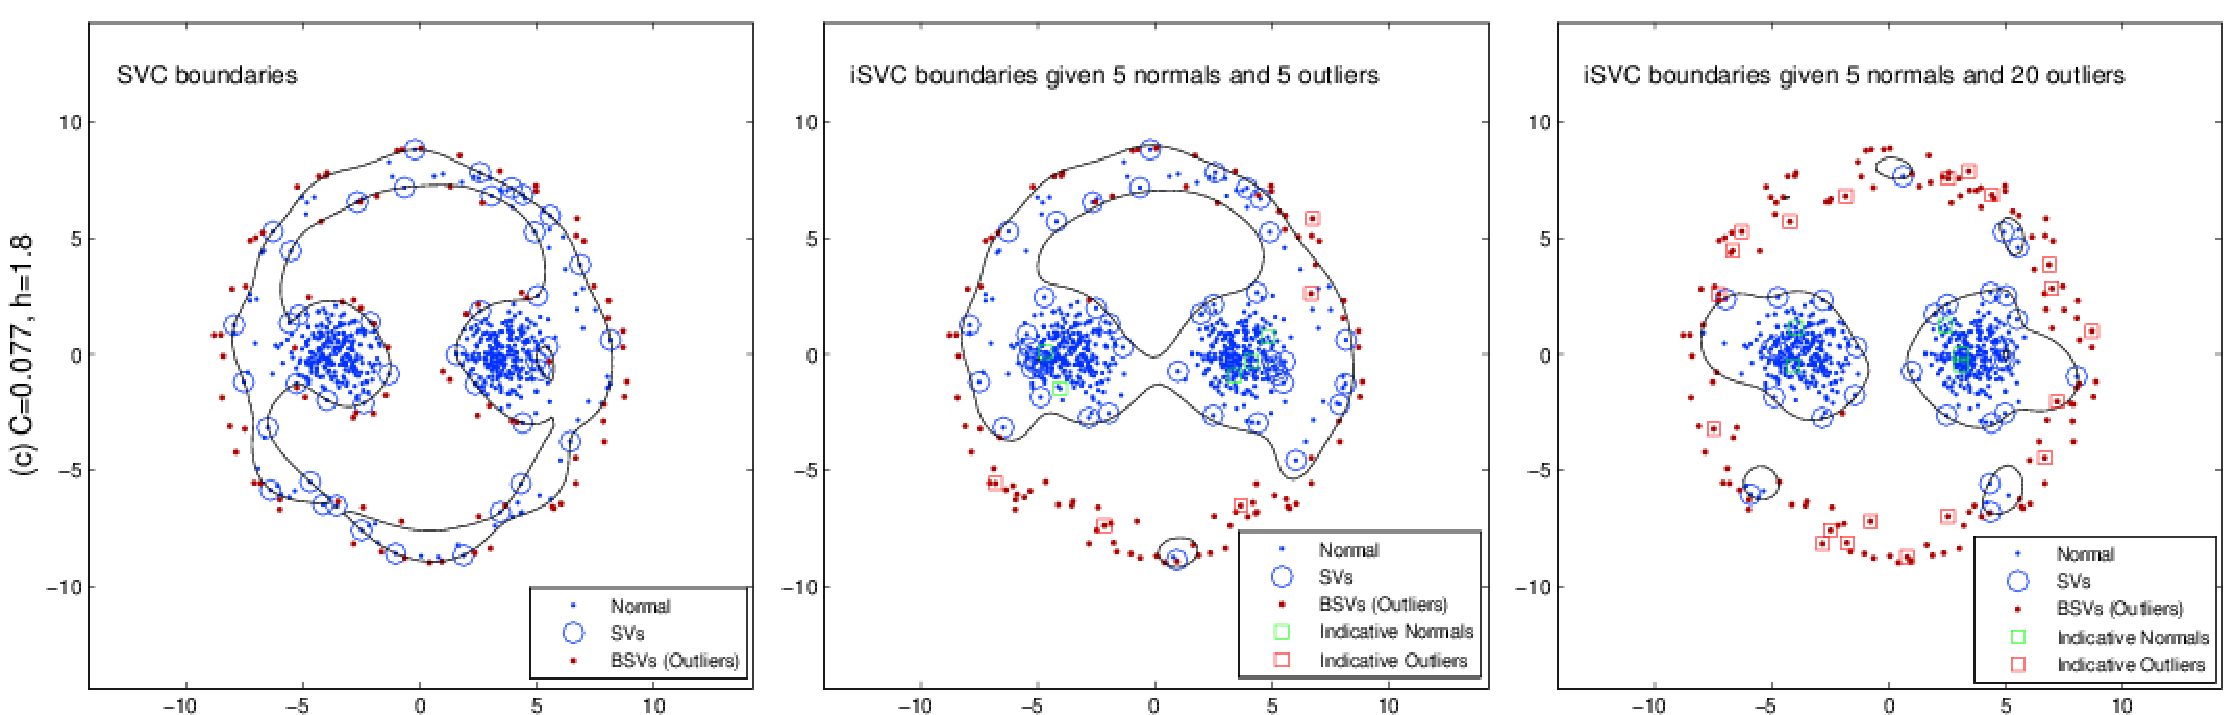
\includegraphics[scale=0.5\textwidth]{imgs/syn_01_03}
\end{figure}
\end{frame}

\subsection{Real-world data set experiments}
\begin{frame}{On digits recognition data set}
\begin{itemize}
\item MINST digit images data set
\item Digits {2,6,9}, 150 images of each
\item 100 digit {0} tampered manually as outliers
\end{itemize}
\begin{figure}
\centering
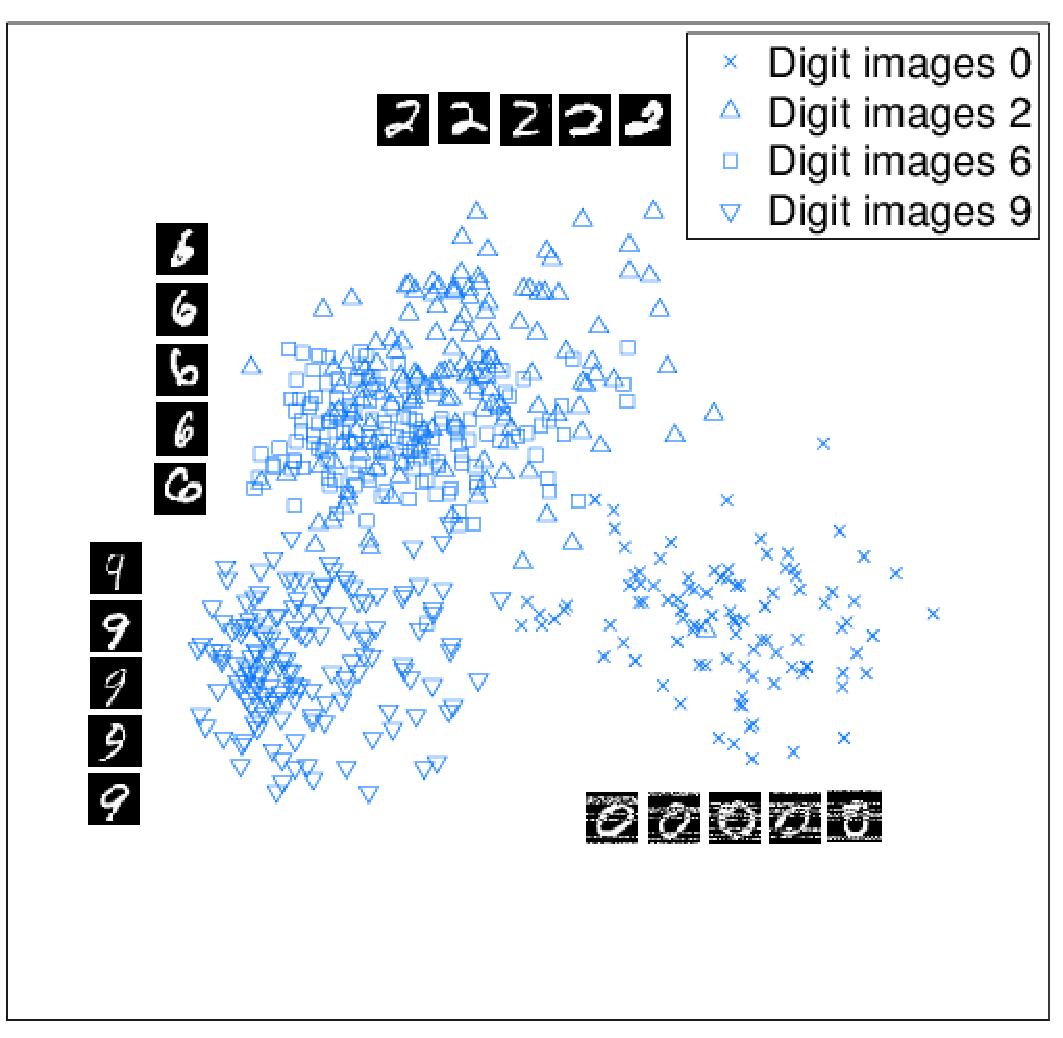
\includegraphics[scale=0.198]{imgs/real_01_01.pdf}
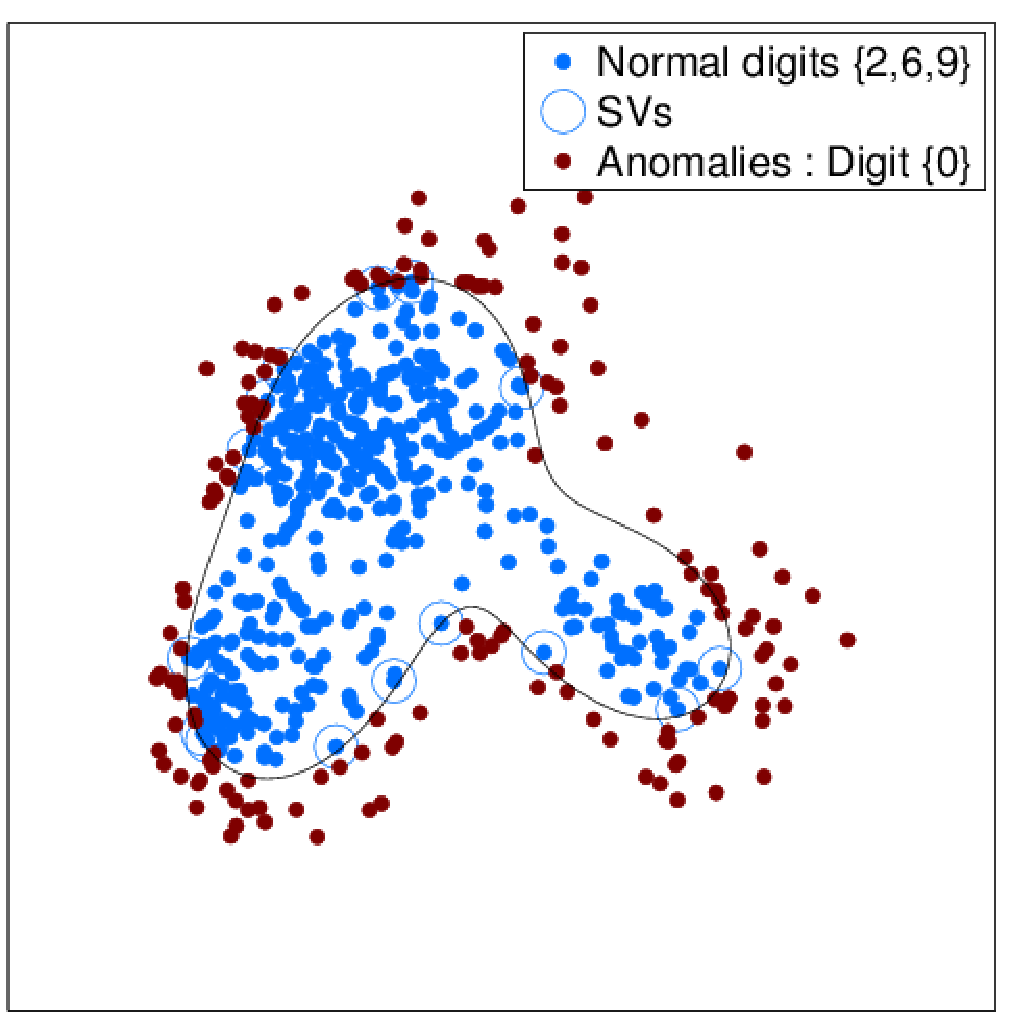
\includegraphics[scale=0.2]{imgs/real_01_02.pdf}
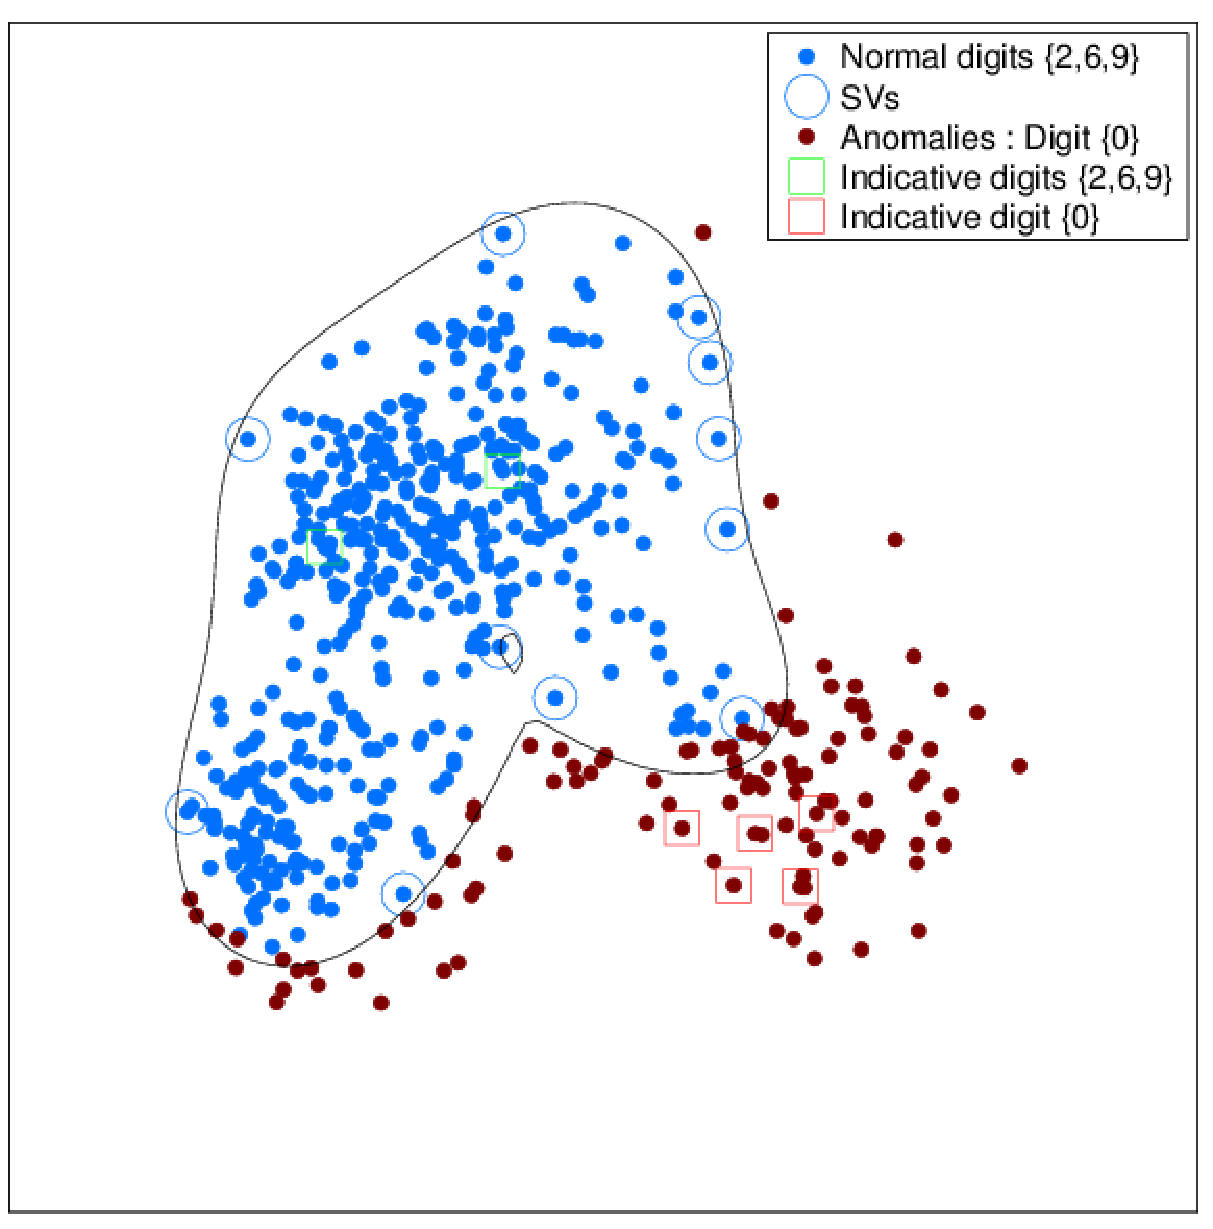
\includegraphics[scale=0.167]{imgs/real_01_03.pdf}
\end{figure}
\end{frame}
\begin{frame}{Numerical evaluation}
\begin{figure}
\centering
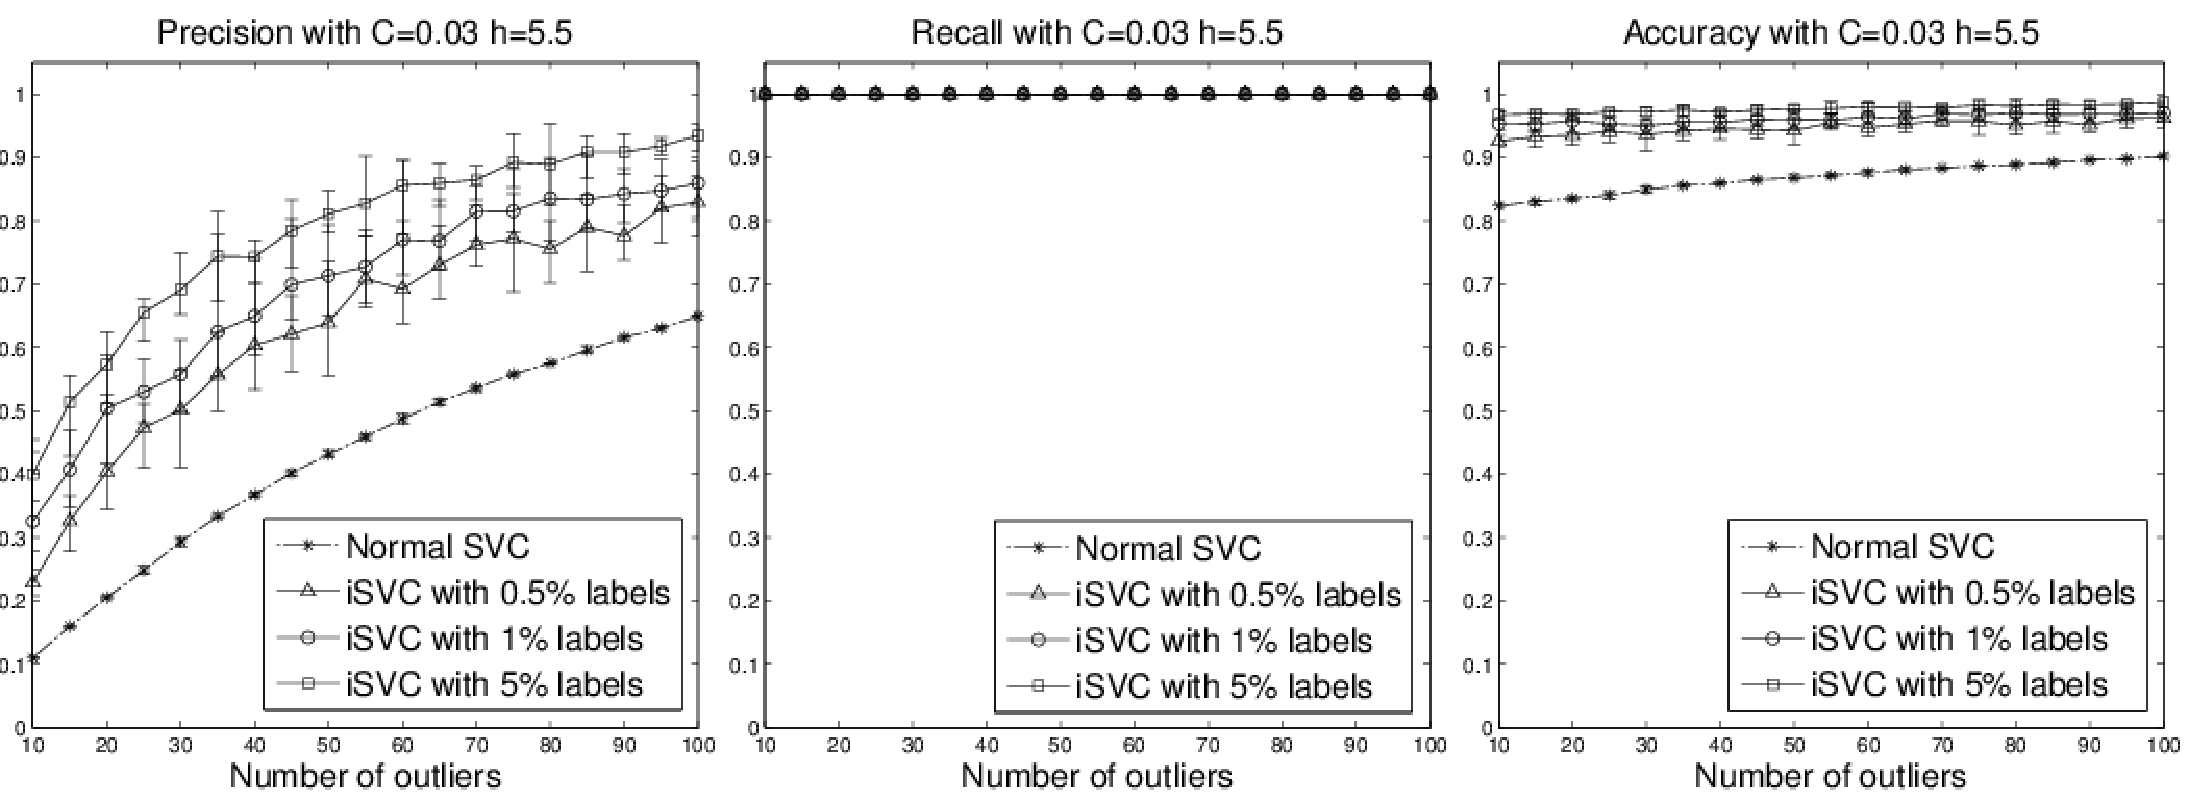
\includegraphics[scale=0.25]{imgs/real_02.pdf}\\
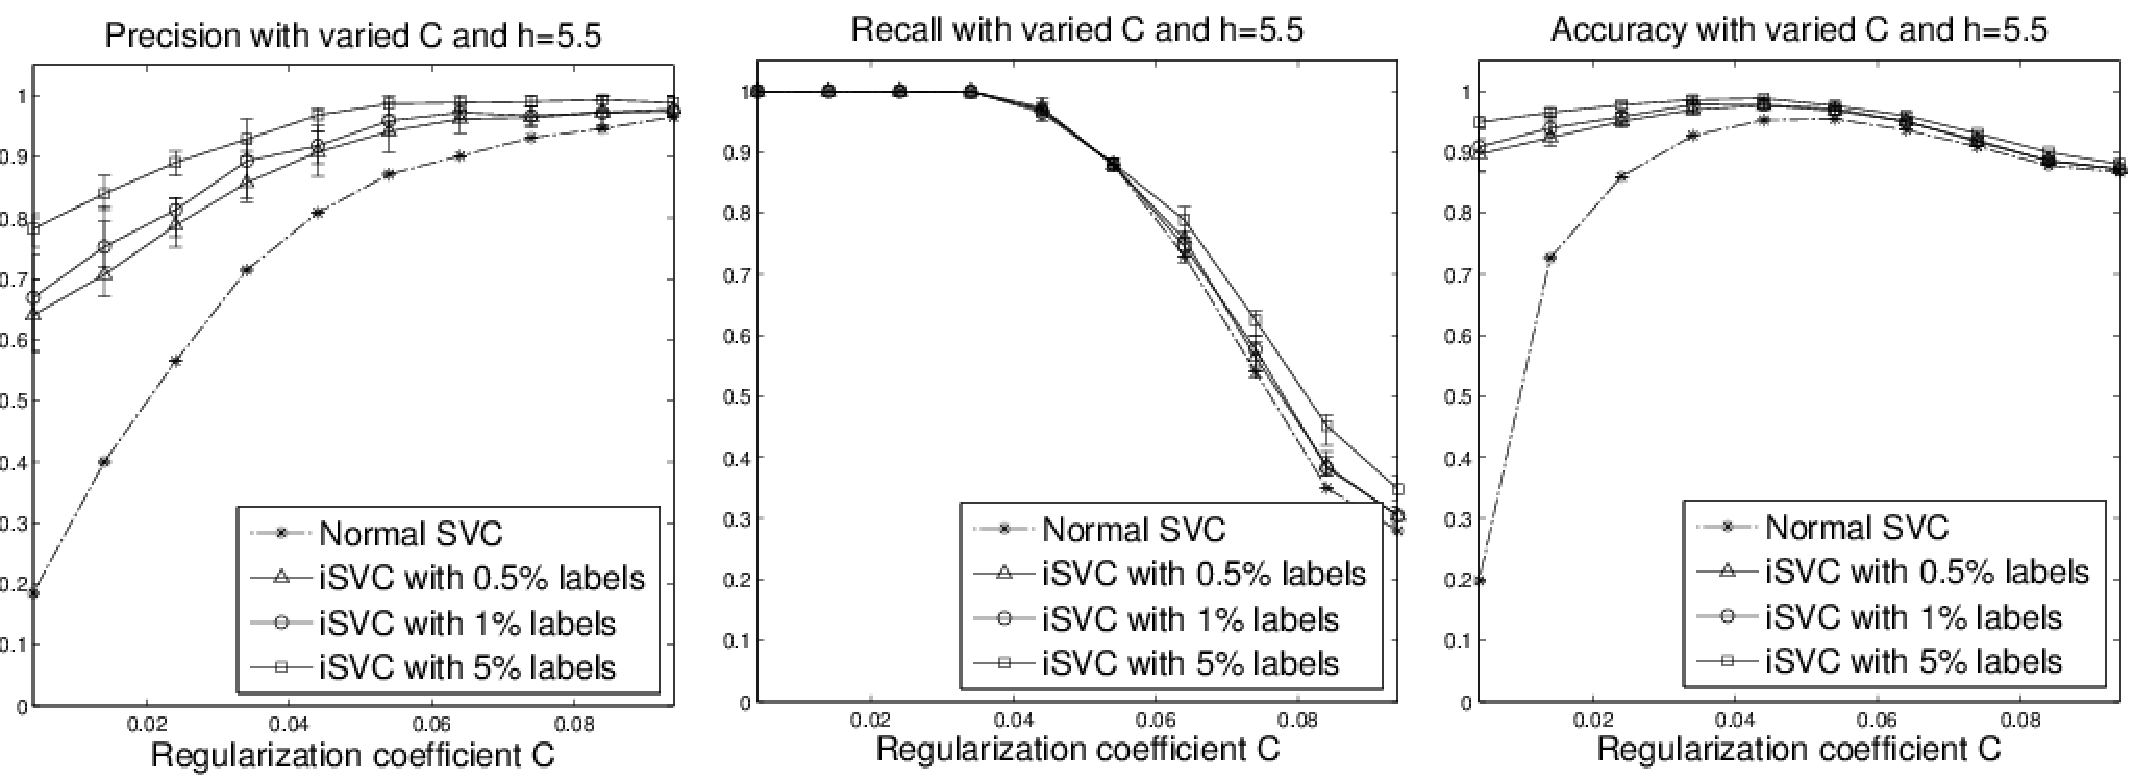
\includegraphics[scale=0.25]{imgs/real_03.pdf}
\end{figure}
\end{frame}
\begin{frame}{On the WDBC data set}
\begin{itemize}
\item Wisconsin Diagnostic Breast Cancer (WDBC) data set
\item 569 samples, out of which 212 are malignant and 357 are benign
\item Test it against semi-supervised fast linear SVM given various labels
\end{itemize}
\end{frame}
\begin{frame}{Results}
\begin{table}[!t]
\small
\setlength{\tabcolsep}{10pt}
% increase table row spacing, adjust to taste
\renewcommand{\arraystretch}{1.3}
% if using array.sty, it might be a good idea to tweak the value of
% \extrarowheight as needed to properly center the text within the cells
%\caption{Empirical results on the WDBC data set given different proportions of sample labels.}
\label{tbl:real_03}
\centering
% Some packages, such as MDW tools, offer better commands for making tables
% than the plain LaTeX2e tabular which is used here.
\begin{tabular}{|c||c|c|c|c|}
\hline
& \multicolumn{4}{c|}{\textbf{WDBC data set with $\mathbf{h=0.9, C=0.001}$}}\\
\cline{2-5}
& Accuracy & $F_1$-measure & FPR & FNR \\
\hline
\textit{SVC} & $63.4\%$ & $50.5\%$ & $28.6\%$ &$50\%$ \\\hline
& \multicolumn{4}{c|}{$5\%$ \textit{positive} and $0\%$ \textit{negative} labels}\\
\hline
\textit{iSVC} & $\mathbf{90.5\%}$ & $\mathbf{87.0\%}$ & $\mathbf{6.4\%}$ &$14.6\%$ \\\hline
\textit{S3VM} & $39.2\%$ & $55.0\%$ & $96.9\%$ &$\mathbf{0\%}$ \\\hline
& \multicolumn{4}{c|}{$0\%$ \textit{positive} and $5\%$ \textit{negative} labels}\\
\hline
\textit{iSVC} & $\mathbf{89.8\%}$ & $\mathbf{87.7\%}$ & $14.8\%$ &$2.4\%$ \\\hline
\textit{S3VM} & $64.9\%$ & $10.7\%$ & $\mathbf{0\%}$ &$94.3\%$ \\\hline
& \multicolumn{4}{c|}{$5\%$ \textit{positive} and $5\%$ \textit{negative} labels}\\
\hline
\textit{iSVC} & $\mathbf{92.3\%}$ & $\mathbf{89.8\%}$ & $\mathbf{7.0\%}$ &$8.9\%$ \\\hline
\textit{S3VM} & $88.4\%$ & $86.3\%$ & $17.4\%$ &$\mathbf{1.9\%}$ \\\hline
& \multicolumn{4}{c|}{$10\%$ \textit{positive} and $10\%$ \textit{negative} labels} \\
\hline
\textit{iSVC} & $\mathbf{93.9\%}$ & $\mathbf{91.9\%}$ & $\mathbf{6.4\%}$ &$5.6\%$ \\\hline
\textit{S3VM} & $92.4\%$ & $90.6\%$ & $10.4\%$ &$\mathbf{2.8\%}$ \\\hline
\end{tabular}
\end{table}
\end{frame}
%\begin{frame}{Statistical Implication}
%\begin{block}{Reichenbach's \textit{Common Cause Principle}}
%If $X$ and $Y$ are correlated, then either $X$ causes $Y$ or $Y$ causes $X$ or they share a latent common cause $Z$.
%\end{block}
%\begin{figure}
%\setcounter{subfigure}{0}
%	\centering
%	\begin{subfigure}[H]{0.3\textwidth}
%		\centering
%		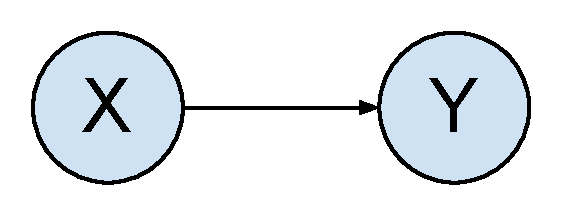
\includegraphics[scale=0.3]{imgs/x2y}
%		\caption{$X$ causes $Y$}
%		%\label{}	
%	\end{subfigure}
%	\begin{subfigure}[H]{0.3\textwidth}
%		\centering
%		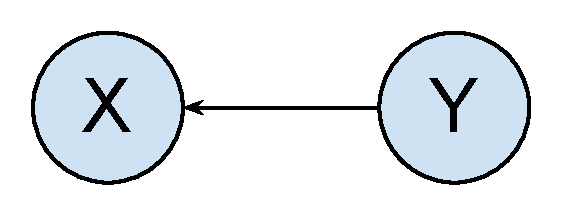
\includegraphics[scale=0.3]{imgs/y2x}
%		\caption{$Y$ causes $X$}
%		%\label{}	
%	\end{subfigure}
%	\begin{subfigure}[H]{0.3\textwidth}
%		\centering
%		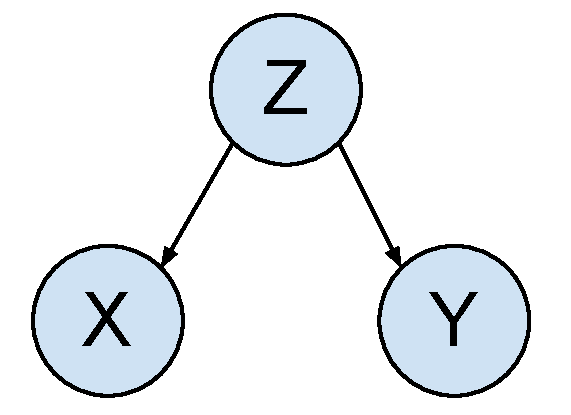
\includegraphics[scale=0.3]{imgs/z2xy}
%		\caption{A common latent cause $Z$}
%		%\label{}	
%	\end{subfigure}
%\end{figure}\pause
%\begin{itemize}
%\item<+-|alert@+> It links causality with probability
%\end{itemize}
%\end{frame}
%\begin{frame}{Functional Causal Model (pearl et al.)} 
%\begin{itemize}[<+->]
%\item A set of variables (factors) $\left\lbrace X_1,\ldots,X_n \right\rbrace$
%\item Directed acyclic graph $\mathcal{G}$ with vertices $\left\lbrace X_1,\ldots,X_n \right\rbrace$
%\item Parents of node $X_i$ in $\mathcal{G}$ are its direct causes
%\item $X_i=f_i(Parents(X_i),\epsilon_i)$, where $\left\lbrace\epsilon_1,\ldots,\epsilon_n\right\rbrace$ are jointly independent noises
%\item The above entails a joint probability distribution $P(X_1,\ldots,X_n)$
%\item Problems are twofold:
%      \begin{enumerate}
%		\item How is the $P$ like?
%		\item Can we recover $\mathcal{G} from P$? 
%	\end{enumerate}
%\item[] \begin{textblock*}{200mm}(0.6\textwidth,-2cm)
%		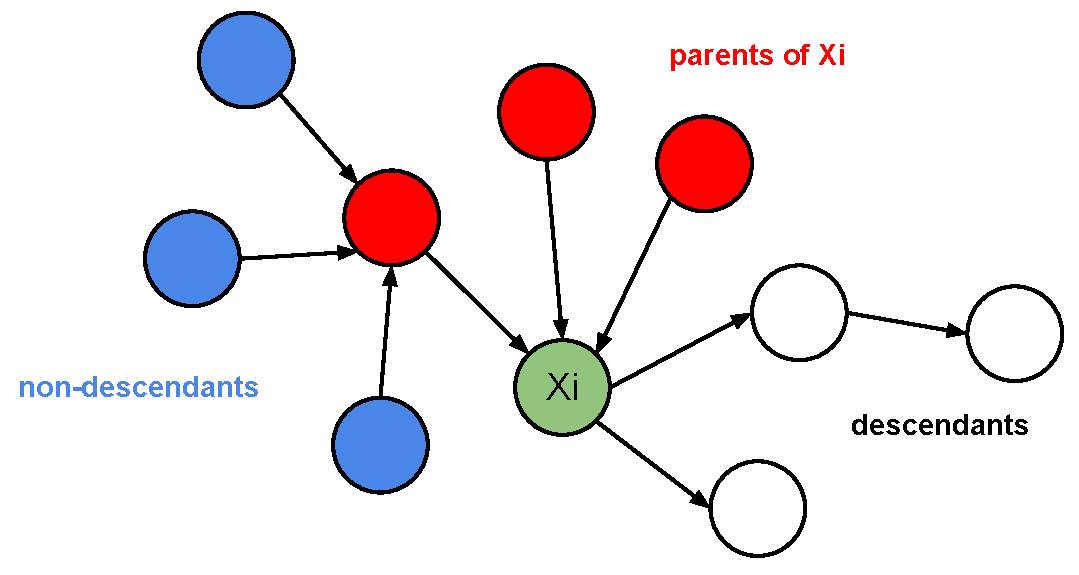
\includegraphics[scale=0.25]{imgs/causalgm}
%	\end{textblock*}
%\end{itemize}
%\end{frame}
%\begin{frame}{Functional Causal Model, ctd.}
%The following are equivalent:
%\begin{itemize}
%\item A functional causal model exists
%\item Local causal Markov condition: $X_i$ is statistically independent of its non-descendants given $X_i$'s parents
%\item Global Causal Markov condition: \textbf{d-separation} characterize the set of independences over all the observables
%\item Factorization: $P(X_1,\ldots,X_n)=\prod_iP(X_i\,|\,Parents(X_i))$
%\end{itemize}
%\end{frame}
%\begin{frame}{Learning causation from Data?}
%\begin{block}{Question}
%Given observational data, can we infer $\mathcal{G}$?
%\end{block}
%\begin{itemize}
%\item \textbf{Simple answer:} impossible without additional information
%\item Possible with interventions (outside force, empirical treatment, etc.)
%\item By conditional independence tests, \textit{Markov equivalence class} containing $\mathcal{G}$ can be learned. \alert{But}, it fails in simplest 2-nodes case.
%\item 2-nodes case can be tackled applying residual dependence test. (see Hoyer et al.)
%\end{itemize}
%\end{frame}
%\begin{frame}{Markov Equivalence Class}
%\textbf{Simplest case with three variables}
%\begin{itemize}
%\item[]<1-> \begin{figure}
%\setcounter{subfigure}{0}
%			\begin{subfigure}[H]{0.4\textwidth}
%			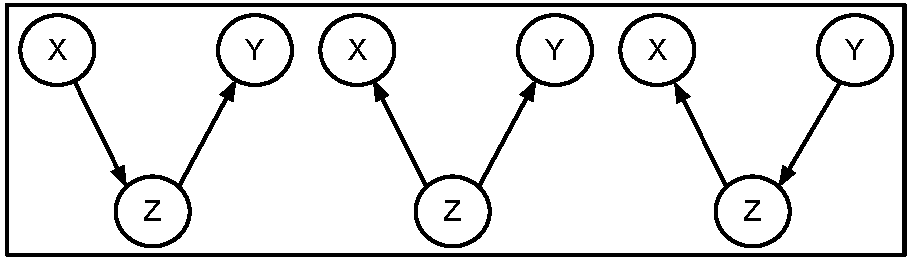
\includegraphics[scale=0.4]{imgs/eqv}
%			\caption{Equivalence}
%			\end{subfigure}\hfill
%			\begin{subfigure}[H]{0.3\textwidth}
%			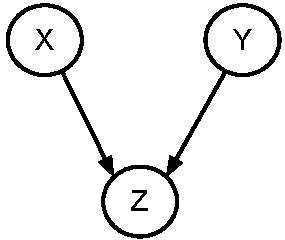
\includegraphics[scale=0.4]{imgs/noneqv}
%			\caption{Non-equivalence}
%			\end{subfigure}
%		\end{figure}
%\item<2-> Samples can be explained by all graphs in equivalence class
%\item<3-> For example:
%\begin{table}
%\centering
%\begin{tabular}{|c|c|}
%\hline
%Equivalence class & Non-equivalence class \\\hline
%$Dep(X,Z\,|\,\emptyset)$ & $Dep(X,Z\,|\,\emptyset)$\\\hline
%$Dep(Y,Z\,|\,\emptyset)$ & $Dep(Y,Z\,|\,\emptyset)$\\\hline
%$Dep(X,Y\,|\,\emptyset)$ & \alert{$Ind(X,Y\,|\,\emptyset)$}\\\hline
%$Ind(X,Y\,|\,Z)$ & \alert{$Dep(X,Y\,|\,Z)$}\\\hline
%\end{tabular}
%\end{table}	
%\end{itemize}
%\end{frame}